\chapter{Основные соотношения}\label{ch:BasicRelations} 

\section{Определение нелокального оператора}\label{sec:BasicRelations/NonlocalOperator}

Определим линейный интегральный оператор $\mathcal{N}$, который представим в виде взвешенной суммы, где первое слагаемое --- это подставляемое в оператор выражение с весовым множителем $p_1$, а второе --- это же выражение, но взвешенное по области $S'(\boldsymbol{x})$ с весовой функцией $\varphi$ и весовым параметром $p_2$,
\begin{gather}
	\label{eq:IntegroDiffOperator}
	\mathcal{N} [f(\boldsymbol{x})] = 
	p_1 f(\boldsymbol{x}) + 
	p_2 \int\limits_{S'(\boldsymbol{x}') \cap S} 
		\varphi(\boldsymbol{x}, \boldsymbol{x}') f(\boldsymbol{x}')
	dS'(\boldsymbol{x}'),
	\quad
	\boldsymbol{x}' \in S'(\boldsymbol{x}).
\end{gather}
Здесь $f(\boldsymbol{x})$ --- выражение, описывающее сохраняющуюся физическую субстанцию;
$p_1 > 0$ и $p_2 \geqslant 0$ --- весовые параметры модели такие, что $p_1 + p_2 = 1$;
$\varphi$~---~функция нелокального влияния, нормированная положительная монотонно убывающая функция в области $S'(\boldsymbol{x})$; 
$\boldsymbol{x}'$ --- точка в области $S'(\boldsymbol{x})$, в которой вычисляется влияние на величины находящиеся в точке $\boldsymbol{x}$;
$S'(\boldsymbol{x})$ --- область нелокального влияния с центром в точке $\boldsymbol{x} \in S$;
$S$ --- область занимаемая рассматриваемым телом.

Отметим, что для каждого отдельно взятого физического процесса $\mathcal{F}$ можно определить свой собственный оператор $\mathcal{N}_\mathcal{F}$ со своим набором весовых констант $p_1$ и $p_2$, функцией нелокального влияния $\varphi$ и областью нелокального влияния $S'(\boldsymbol{x})$. Однако для упрощения дальнейших выкладок, без потери общности, ограничимся гипотезой, что для тепловых и механических моделей параметры нелокальности одинаковые.

\section{Уравнение стационарной теплопроводности}\label{sec:BasicRelations/HeatEquation}

В произвольной замкнутой области $S \subset \mathbb{R}^2$ с кусочно-гладкой границей $\partial S$ уравнение стационарной теплопроводности имеет вид \cite{MSS}
\begin{gather}
	\label{eq:StationaryHeatEquation}
	\nabla \cdot \boldsymbol{q} = q_V,
\end{gather}
где $q_V$ --- объёмная плотность мощности внутренних источников и стоков теплоты;
$\boldsymbol{q}$ --- вектор плотности теплового потока, который определим как обобщение гипотезы Био --- Фурье \cite{ThermoViscoElasticity1, ThermoViscoElasticity2, ThermoViscoElasticity3}, подставив её в \mbox{оператор~(\ref{eq:IntegroDiffOperator})}
\begin{gather}
	\label{eq:BiotFourier}
	\boldsymbol{q}(\boldsymbol{x}) = 
	\mathcal{N} \left( -\widehat{\boldsymbol{\lambda}} \cdot \nabla T \right),
\end{gather}
где $\widehat{\boldsymbol{\lambda}} = \lambda_{ij} \boldsymbol{e}_i \otimes \boldsymbol{e}_j$ --- тензор коэффициентов теплопроводности;
$T = T(\boldsymbol{x})$ --- поле температуры.

Граничные условия первого, второго и третьего родов для уравнения (\ref{eq:StationaryHeatEquation}) имеют вид \cite{MSS}
\begin{gather}
	\label{eq:ThermalBoundaries}
	T|_{\Gamma_1} = T_{\Gamma} (\boldsymbol{x}),
	\quad
	\boldsymbol{n} \cdot \boldsymbol{q}|_{\Gamma_2} = f(\boldsymbol{x}),
	\quad
	\boldsymbol{n} \cdot \boldsymbol{q}|_{\Gamma_3} = \alpha (T_a(\boldsymbol{x}) - T(\boldsymbol{x}))),
\end{gather}
где $\Gamma_1 \cup \Gamma_2 \cup \Gamma_3 = \partial S$, $\Gamma_1 \cap \Gamma_2 = \Gamma_1 \cap \Gamma_3 = \Gamma_2 \cap \Gamma_3 = \varnothing$;
$T_{\Gamma} (\boldsymbol{x})$ и $f(\boldsymbol{x})$ --- функции, задающие температуру и плотность теплового потока на границах $\Gamma_1$ и $\Gamma_2$ соответственно;
$\alpha$ --- коэффициент конвективного теплообмена с внешней средой;
$T_a (\boldsymbol{x})$ --- температура внешней среды вблизи границы $\Gamma_3$.
Для простоты дальнейшего изложения будем предполагать, что функции $T_{\Gamma}(\boldsymbol{x})$, $f(\boldsymbol{x})$ и $T_a(\boldsymbol{x})$ равны нулю во множествах, где они не определены.

\section{Уравнение равновесия}\label{sec:BasicRelations/EquilibriumEquation}

В произвольной замкнутой области $S \subset \mathbb{R}^2$ с кусочно-гладкой границей $\partial S$ определим уравнение равновесия сплошной среды \cite{MSS}
\begin{gather}
	\label{eq:EquilibriumEquation}
    \nabla \cdot \widehat{\boldsymbol{\sigma}} = \boldsymbol{b},
\end{gather}
где $\boldsymbol{b} = b_i \boldsymbol{e}_i$ --- вектор плотности объёмных сил;
$\widehat{\boldsymbol{\sigma}} = \sigma_{ij} \boldsymbol{e}_i \otimes \boldsymbol{e}_j$ --- тензор напряжений. В работе рассматриваем случай несвязанной термоупругой задачи, поэтому определим тензор напряжений $\widehat{\boldsymbol{\sigma}}$ через обобщение закона Дюамеля~---~Неймана с использованием оператора (\ref{eq:IntegroDiffOperator}) \cite{ThermoViscoElasticity1, ThermoViscoElasticity2, ThermoViscoElasticity3}
\begin{gather}
	\label{eq:DuamelNeumann}
	\widehat{\boldsymbol{\sigma}}(\boldsymbol{x}) =
	\mathcal{N} \left(
		\widehat{\text{\textbf{C}}} \cdot \cdot 
		\left( \widehat{\boldsymbol{\varepsilon}} - \widehat{\boldsymbol{\alpha}}^T \Delta T \right)
	\right).
\end{gather}
Здесь \mbox{$\widehat{\varepsilon} = \varepsilon_{ij} \boldsymbol{e}_i \otimes \boldsymbol{e}_j$}~---~тензор деформации;
$\widehat{\text{\textbf{C}}} = C_{ijkl} \boldsymbol{e}_i \otimes \boldsymbol{e}_j \otimes \boldsymbol{e}_k \otimes \boldsymbol{e}_l$ --- тензор коэффициентов упругости;
$\widehat{\boldsymbol{\alpha}}^T = \alpha_{ij}^T \boldsymbol{e}_i \otimes \boldsymbol{e}_j$ --- тензор температурных коэффициентов линейного расширения;
$\Delta T = T - T_0$ --- разница между текущим распределением температуры $T$ и распределением $T_0$ при котором отсутствуют температурные деформации.

Далее будем считать, что тело является линейно-упругим и изотропным. В случае плоского напряжённого состоянии, компоненты тензора упругости $\widehat{\text{\textbf{C}}}$ будут определены следующим образом \cite{MSS}
\begin{gather*}
	C_{ijkl} =
	\dfrac{\nu E}{1 - \nu^2} \delta_{ij} \delta_{kl} +
	\dfrac{E}{2(1 + \nu)} (\delta_{ik} \delta_{jl} + \delta_{il} \delta_{jk}),
\end{gather*}
где $E$ --- модуль Юнга;
$\nu$ --- коэффициент Пуассона;
$\delta_{ij}$ --- дельта Кронекера.
Если же рассмотрен случай плоского деформированного состояния, то компоненты тензора упругости имеют аналогичную форму записи
\begin{gather*}
	C_{ijkl} =
	\dfrac{\widetilde{\nu} \widetilde{E}}{1 - \widetilde{\nu}^2} \delta_{ij} \delta_{kl} +
	\dfrac{\widetilde{E}}{2(1 + \widetilde{\nu})} (\delta_{ik} \delta_{jl} + \delta_{il} \delta_{jk}),
\end{gather*}
однако, здесь $\widetilde{E} = E / (1 - \nu^2)$ и $\widetilde{\nu} = \nu / (1 - \nu)$. Также будем считать, что тело расширяется равнонаправлено, поэтому тензор температурных коэффициентов линейного расширения будет диагональным и иметь всего один коэффициент $\alpha^T$, то есть \cite{MSS}
\begin{gather*}
	\widehat{\boldsymbol{\alpha}}^T = \alpha^T \widehat{\text{\textbf{I}}}_2.
\end{gather*}

Примем гипотезу, что деформации достаточно малы, поэтому для определения компонент тензора деформации $\widehat{\boldsymbol{\varepsilon}}$ воспользуемся соотношениями \mbox{Коши \cite{MSS}}
\begin{gather*}
	\widehat{\boldsymbol{\varepsilon}} = 
	\dfrac{\boldsymbol{u} + (\nabla \boldsymbol{u})^T}{2} = 
	\dfrac{u_{i, j} + u_{j, i}}{2} \boldsymbol{e}_i \otimes \boldsymbol{e}_j,
\end{gather*}
где $\boldsymbol{u}$ --- вектор перемещения.

Будем рассматривать граничные условия первого и второго родов \cite{MSS}, также именуемые кинематическими и силовыми соответственно,
\begin{gather}
	\label{eq:StressBoundaries}
	\boldsymbol{u}|_{\Gamma_4} = \boldsymbol{d} (\boldsymbol{x}),
	\quad
	\boldsymbol{n} \cdot \widehat{\boldsymbol{\sigma}}|_{\Gamma_5} = \boldsymbol{p} (\boldsymbol{x}),
\end{gather}
где $\boldsymbol{d} (\boldsymbol{x}) = d_i (\boldsymbol{x}) \boldsymbol{e}_i$ --- вектор перемещений на границе $\Gamma_4$;
$\boldsymbol{p} (\boldsymbol{x}) = p_i (\boldsymbol{x}) \boldsymbol{e}_i$ --- вектор плотности поверхностностного нагружения на границе $\Gamma_5$. Помимо этого будем рассматривать комбинированные граничные условия, когда по одной компоненте задано перемещение, а по другой поверхностное нагружение. Как и в случае с граничными условиями уравнения теплопроводности, для простоты будем считать, что функции задающие граничные условия уравнения равновесия (\ref{eq:DuamelNeumann}) будут равны нулю на границах, на которых они не определены.

\section{Определение области и функции нелокальности}\label{sec:BasicRelations/InfluenceFunction}

В определении оператора (\ref{eq:IntegroDiffOperator}) нет ограничения на выбор области нелокального влияния $S'(\boldsymbol{x})$. Она  может быть как неограниченной и включать в себя всю расчётную область, так и замкнутой, покрывая лишь часть рассматриваемого тела. В любом случае, выбор области $S'(\boldsymbol{x})$ подразумевает так же и выбор функции нелокального влияния $\varphi$. С практической точки зрения, следует выбирать такую функцию $\varphi$, чтобы интеграл от неё по области $S'(\boldsymbol{x})$ был в рамках заданной точности близким к единице \cite{Eringen3}. Вместе с этим область $S'(\boldsymbol{x})$ должна быть достаточной для аппроксимации наблюдаемых явлений, но в то же время, она не должна покрывать всю область занимаемую телом, так как на практике при аппроксимации уравнений это позволит использовать разреженные матрицы для хранения коэффициентов СЛАУ \cite{Pisanetzkiy} и значительно облегчит численные расчёты, повысив общую эффективность использования вычислительных ресурсов. 

Выбор области нелокального влияния $S'(\boldsymbol{x})$ является нетривиальной задачей, где в первую очередь стоит опираться на структуру рассматриваемого материала \cite{Eringen3}. Поэтому рассмотрим наиболее общий (пусть и не исчерпывающий) случай и представим $S'(\boldsymbol{x})$ в виде фигуры ограниченной кривой Ламэ \cite{Superellipse}, изображённой на Рис.~\ref{fig:SuperEllipse} при различных параметрах $n > 0$. У такого семейства фигур есть также параметры, отвечающие за длины главных полуосей $r_1 > 0$ и $r_2 > 0$. На основе этих параметров можем определить метрическую функцию
\begin{gather}
	\label{eq:metricFunction}
	\rho_n(\boldsymbol{x}, \boldsymbol{x}') = 
	\left(
		\left| \dfrac{x_1 - x_1'}{r_1} \right|^n +
		\left| \dfrac{x_2 - x_2'}{r_2} \right|^n
	\right)^{\dfrac{1}{n}},
\end{gather}
использовав которую приступим к построению всевозможных функций нелокального влияния $\varphi$, соблюдая правило, что функция $\varphi$ должна монотонно убывать по мере роста функции $\rho_n$.

\begin{figure}[ht]
    \centerfloat{
        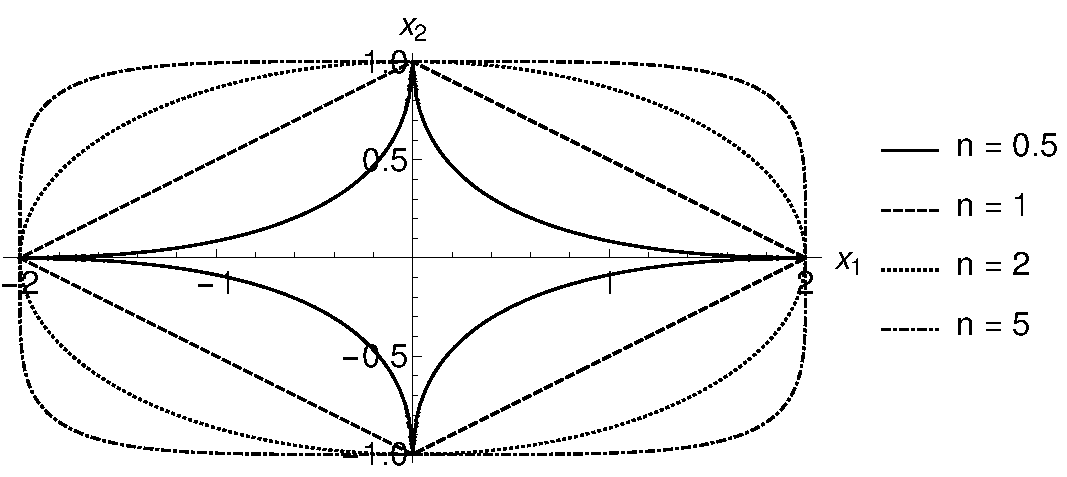
\includegraphics[width=0.85\textwidth]{pics/SuperEllipse.pdf}
    }
    \caption{Кривые Ламэ при различных параметрах $n$}\label{fig:SuperEllipse}
\end{figure}

Воспользовавшись метрической функцией $\rho_n$ (\ref{eq:metricFunction}), построим семейство полиномиальных функций нелокального влияния, определённых в ограниченной области \cite{PolyInfluence},
\begin{gather}
	\label{eq:polynomialInfluence}
	\varphi_{p,q}^{P}(\boldsymbol{x}, \boldsymbol{x}') =
	\begin{cases}
		A(1 - \rho_n(\boldsymbol{x}, \boldsymbol{x}')^p)^q, \quad &\rho_n(\boldsymbol{x}, \boldsymbol{x}') \leqslant 1, \\
		0, &\rho_n(\boldsymbol{x}, \boldsymbol{x}') > 1,
	\end{cases}
\end{gather}
где $p > 0$ и $q > 0$ --- параметры управляющие плотностью распределения функции; $A$ --- нормирующий множитель. Для определения нормирующего множителя $A$ проведём нормировку области $S'(\boldsymbol{x})$ вдоль каждой из осей таким образом, чтобы исключить параметры $r_1$ и $r_2$ из метрической функции $\rho_n$ (\ref{eq:metricFunction}). Далее на получившейся безразмерной области $\widetilde{S}'(\widetilde{\boldsymbol{x}}')$ введём аналог полярной системы координат с обобщением на параметр $n$, где координату радиуса $\rho$ и угла $\theta$ вычислим по следующим формулам
\begin{gather*}
	\begin{cases}
		\rho = (|\widetilde{x}_1|^n + |\widetilde{x}_2|^n)^{\frac{1}{n}}, \\
		\theta = \operatorname{arctg} \left( \dfrac{\widetilde{x}_2}{\widetilde{x}_1} \right).
	\end{cases}
\end{gather*}
Тогда обратная зависимость координат принимает вид
\begin{gather*}
	\begin{cases}
		\widetilde{x}_1 = \dfrac{\rho}{\left( 1 + \operatorname{tg}^n (\theta) \right)^{\frac{1}{n}}}, \\
		\widetilde{x}_2 = \dfrac{\rho \operatorname{tg} (\theta)}{\left( 1 + \operatorname{tg}^n (\theta) \right)^{\frac{1}{n}}},
	\end{cases}
\end{gather*}
на основе которой можем вычислить якобиан необходимый для интегрирования внутри области $\widetilde{S}' (\boldsymbol{x})$
\begin{gather*}
	J_n = \det \left(
	\begin{tabular}{cc}
		$\dfrac{\partial \widetilde{x}_1}{\partial \rho}$ & $\dfrac{\partial \widetilde{x}_1}{\partial \theta}$ \\
		$\dfrac{\partial \widetilde{x}_2}{\partial \rho}$ & $\dfrac{\partial \widetilde{x}_2}{\partial \theta}$
	\end{tabular}
	\right) =
	\dfrac{\rho}{\cos^2 \theta \left( 1 + \operatorname{tg}^n (\theta) \right)^{\frac{2}{n}}}.
\end{gather*}
Теперь проинтегрируем по области $\widetilde{S}' (\boldsymbol{x})$ полиномиальную функцию нелокального влияния $\varphi_{p,q}^{P}$ (\ref{eq:polynomialInfluence})
\begin{gather*}
	\int\limits_0^{2\pi} \int\limits_0^1 A (1 - \rho_n^p)^q J_n d\rho d\theta = 1,
\end{gather*}
откуда, перейдя обратно к размерной области $S'(\boldsymbol{x})$, можем установить, что величина нормировочного параметра $A$ равна выражению
\begin{gather*}
	A = \dfrac{np}
	{
		4 r_1 r_2 
		\operatorname{B}\left( \dfrac{1}{n}, \dfrac{1}{n} \right) 
		\operatorname{B}\left( \dfrac{2}{p}, q+1 \right)
	},
\end{gather*}
где $\operatorname{B}$ --- бета функция Эйлера \cite{SpecialFunction}.
Отдельно отметим, что при стремлении параметра $n$ к бесконечности, нормировочный множитель принимает значение
\begin{gather*}
	A = \dfrac{p}{8 r_2 r_2 \operatorname{B}\left( \dfrac{2}{p}, q+1 \right)},
\end{gather*}
а метрическая функция $\rho_n$ (\ref{eq:metricFunction}) вырождается в следующую
\begin{gather}
	\label{eq:metricFunctionInfinity}
	\rho_{\infty} (\boldsymbol{x}, \boldsymbol{x}') = 
	\max \left( 
		\left| \dfrac{x_1 - x_1'}{r_1} \right|,
		\left| \dfrac{x_2 - x_2'}{r_2} \right|
	\right).
\end{gather}
Далее при использовании данного семейства функций, в случае когда длины полуосей $r_1$ и $r_2$ равны, будем обозначать их одним символом $r$ и называть его радиусом нелокальности.

На Рис.~\ref{fig:PolynomialInfluencePortrait} представлены распределения полиномиальных функций нелокального влияния (\ref{eq:polynomialInfluence}) в сечении вдоль оси $x_1$, где показано, что увеличение параметра $p$ делает распределение функции более равномерным и в пределе такое распределение стремится к константе обратно пропорциональной площади заключённой в область $S'(\boldsymbol{x})$. Увеличение параметра $q$ концентрирует распределение в центре области и в пределе распределение стремится к дельта-функции Дирака.

\begin{figure}[ht]
    \begin{minipage}[b][][b]{0.49\linewidth}\centering
        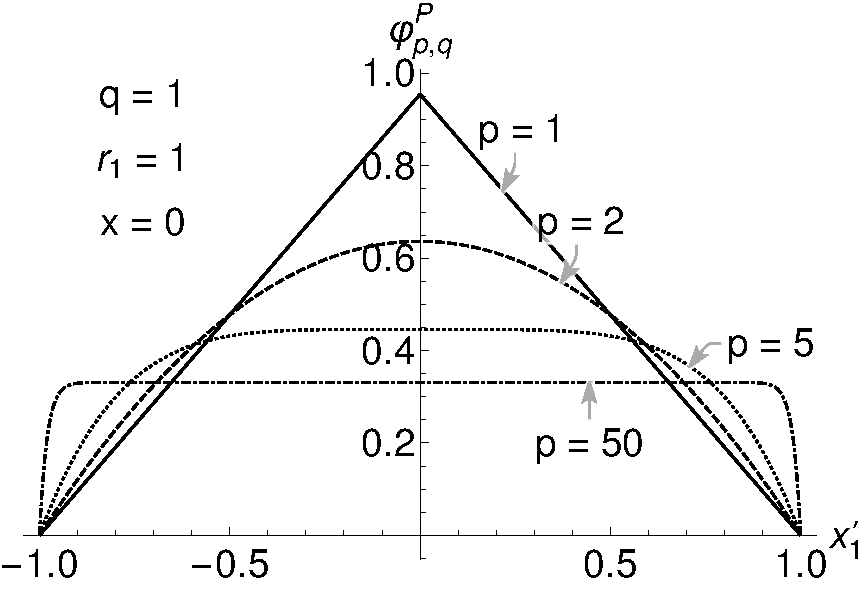
\includegraphics[width=\linewidth]{pics/PolynomialInfluenceP.pdf} \\ а)
    \end{minipage}
    \hfill
    \begin{minipage}[b][][b]{0.49\linewidth}\centering
        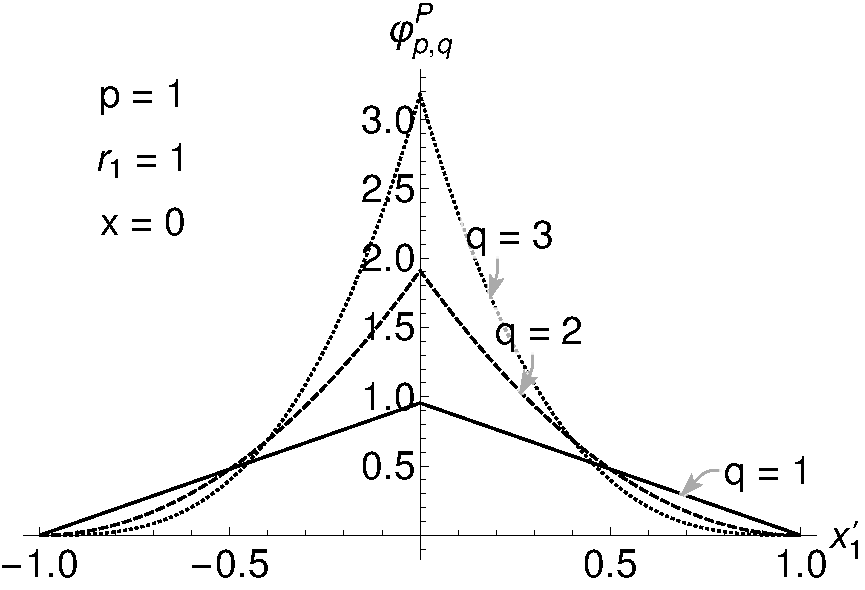
\includegraphics[width=\linewidth]{pics/PolynomialInfluenceQ.pdf} \\ б)
    \end{minipage}
    \caption{Портреты полиномиальных функций влияния в сечении вдоль оси $x'_1$ при вариации (а) параметра $p$ и (б) параметра $q$}
    \label{fig:PolynomialInfluencePortrait}
\end{figure}

Аналогично можем определить семейство экспоненциальных функций, для которых область влияния бесконечная
\begin{gather}
	\label{eq:exponentiallInfluence}
	\varphi_{p,q}^{E} (\boldsymbol{x}, \boldsymbol{x}') =
	A \exp \left(-q\rho_n(\boldsymbol{x}, \boldsymbol{x}')^p \right).
\end{gather}
Параметры $p > 0$ и $q > 0$ --- параметры плотности распределения; $A$ --- нормировочный коэффициент. Для определения параметра $A$ проделаем аналогичную процедуру, которая была рассмотрена в полиномиальном семействе функций, но область интегрирования неограничена, поэтому при переходе в новую систему координат необходимо вычислить несобственный интеграл
\begin{gather*}
	\int\limits_0^{2\pi}
		\int\limits_0^{\infty}
			A \exp \left(-q\rho^p \right) J_n
		d \rho
	d \theta = 1,
\end{gather*}
откуда находим, что значение нормировочного множителя $A$ равно следующему выражению
\begin{gather*}
	\label{eq:normExp}
	A = 
	\dfrac
	{
		4^{\frac{1}{n}} n p q^{\frac{2}{p}}
	}
	{
		8 r_1 r_2 \operatorname{B} \left( \dfrac{1}{2}, \dfrac{1}{n} \right) \operatorname{\Gamma} \left( \dfrac{2}{p} \right)
	},
\end{gather*}
а при стремлении $n$ к бесконечности он принимает следующую форму
\begin{gather*}
	A = \dfrac{p q^{\frac{2}{p}}}{8 r_1 r_2 \Gamma \left( \dfrac{2}{p} \right)},
\end{gather*}
где $\Gamma$ --- гамма-функция \cite{SpecialFunction}. Обратим внимание, что при $q = 0.5$, $p = 2$ и $n = 2$ получаем функцию нормального распределения Гаусса, для которой параметры $r_1$ и $r_2$ можем определить по правилу <<3 сигма>> \cite{TeorVer}. Здесь, как и в случае с полиномиальным семейством функций, в случае равенства $r_1$ и $r_2$, будем обозначать их одним символом $r$, но называть его будем дисперсионным параметром нелокальности.

На Рис.~\ref{fig:ExponentialInfluencePortrait} представлены распределения экспоненциальных функций нелокального влияния (\ref{eq:exponentiallInfluence}) в сечениях вдоль оси $x_1$. Здесь параметры $p$ и $q$ имеют тот же смысл, что и у полиномиального семейства.

\begin{figure}[ht]
    \begin{minipage}[b][][b]{0.49\linewidth}\centering
        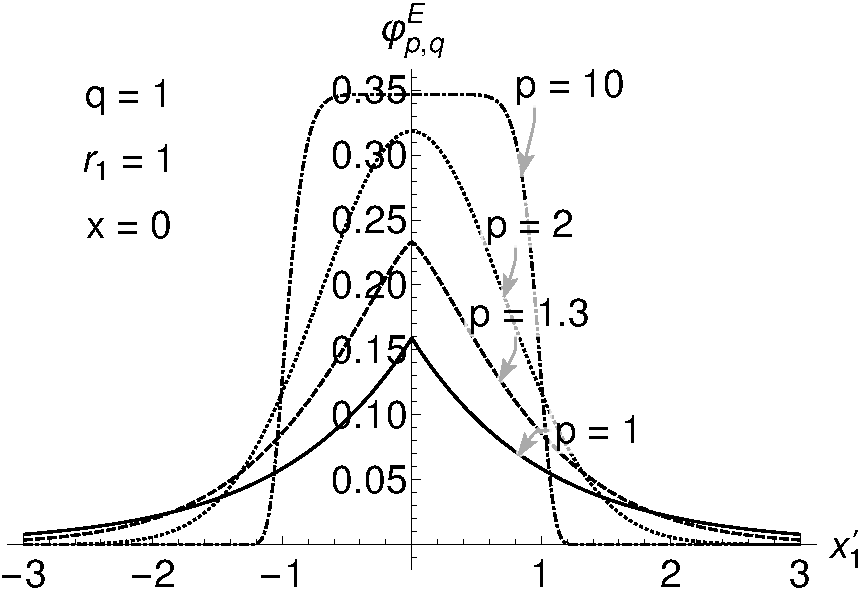
\includegraphics[width=\linewidth]{pics/ExponentialInfluenceP.pdf} \\ а)
    \end{minipage}
    \hfill
    \begin{minipage}[b][][b]{0.49\linewidth}\centering
        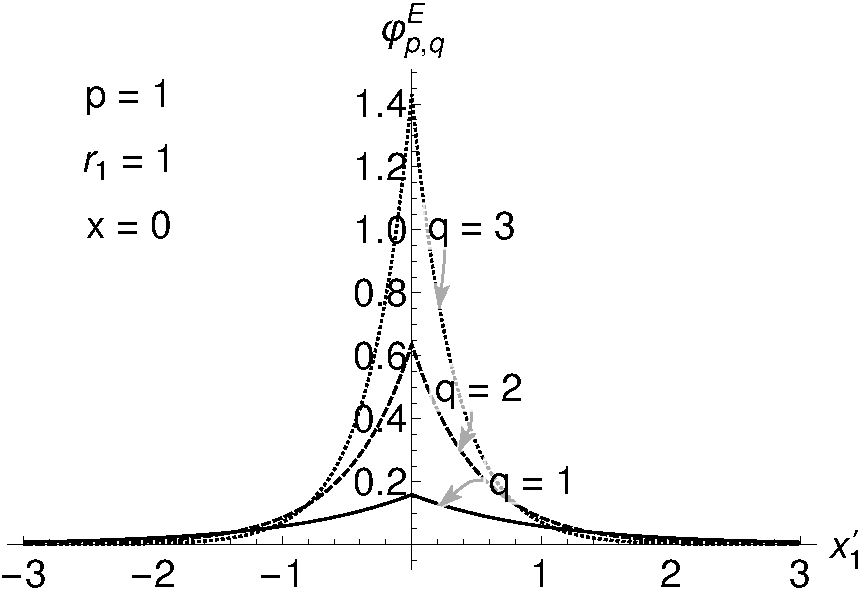
\includegraphics[width=\linewidth]{pics/ExponentialInfluenceQ.pdf} \\ б)
    \end{minipage}
    \caption{Портреты экспоненциальных функций влияния в сечении вдоль оси $x'_1$ при вариации (а) параметра $p$ и (б) параметра $q$}
    \label{fig:ExponentialInfluencePortrait}
\end{figure}

Для экспоненциального семейства функций при заданой ограниченной области $S'(\boldsymbol{x})$ возникает потребность в определении параметров $r_1$ и $r_2$ таких, чтобы нормировка функции была в рамках заданного квантиля $0 < Q < 1$. Для этого снова применим процедуру перехода к обобщённой полярной системе координат, исключим параметры $r_1$ и $r_2$ из метрической функции (\ref{eq:metricFunction}) путём её обезразмеривания, тогда верхний предел интегрирования будем считать переменным и равным $R$
\begin{gather*}
	\int\limits_0^{2\pi}
		\int\limits_0^{R}
			A \exp \left(-q\rho^p \right) J_n
		d \rho
	d \theta = Q.
\end{gather*}
После интегрирования приходим к уравнению
\begin{gather}
	\label{eq:quantil}
	1 - \dfrac{
		\Gamma \left( \dfrac{2}{p}, q R^p \right)
		}{
		\Gamma \left( \dfrac{2}{p} \right)
		} = Q,
\end{gather}
из которого путём численного решения можем найти длину $R$ при заданных параметрах $p$, $q$ и квантиля $Q$. Отметим, что данное уравнение не зависит от параметра $n$, что упрощает анализ при выборе функций влияния. Кроме того в практических расчётах значение параметра $Q$ следует выбирать достато близким к $1$. Так, например, для функции нормального распределения, при условии $Q = 0.99$ получим значение $R = 3.03485$, что соответствует известному правилу <<3 сигма>> \cite{TeorVer}. После нахождения параметра $R$, значения параметров $r_1$ и $r_2$ можем найти просто поделив соответствующую длину полуоси области $S' (\boldsymbol{x})$ на величину $R$.

Отметим, что параметр $q$ в экспоненциальном семействе функций (\ref{eq:exponentiallInfluence}) является избыточным, так как его вариация напрямую связана с параметрами $r_1$ и $r_2$. При подборе параметров $r_1$ и $r_2$ по вышеизложенному алгоритму при различных $q$, распределения функций будут одинаковыми. Однако этот параметр введён намеренно, так как он упрощает управление распределением функций и с некоторыми оговорками будет использован в дальнейших исследованиях при сравнении с полиномиальным семейством функций.

\section{Основные результаты и выводы по главе 1}\label{sec:BasicRelations/Conclusion}

\begin{enumerate}
	\item Определён интегральный нелокальный оператор; с его помощью определены уравнения стационарной теплопроводности и равновесия в нелокальных постановках, которые представлены в интегро-дифференциальной форме.
	
	\item Предложены два семейства функций нелокального влияния: полиномиальное семейство функций, с ограниченной областью определения, и экспоненциальное семейство функций, с неограниченной областью определения.
\end{enumerate}